\documentclass{BscUS}
\usepackage{setspace}
\usepackage{graphicx}
\usepackage{polski}
\usepackage[utf8]{inputenc}
%\usepackage[OT4]{fontenc}
\usepackage{verbatim}
%\usepackage{libertine}
\usepackage{fourier}
\usepackage[T1]{fontenc}
\usepackage{enumitem}
\setitemize{noitemsep,topsep=0pt,parsep=0pt,partopsep=0pt}

\usepackage{amsmath}
\usepackage{gensymb}
\usepackage{physics}
\usepackage{siunitx}
\usepackage{nameref}
\usepackage{listings}

\usepackage{color}

\usepackage{array}

 \usepackage{multirow}
 \usepackage[table,xcdraw]{xcolor}

\usepackage{fancyvrb}
\DefineVerbatimEnvironment{packet}{Verbatim}{xleftmargin=40mm,baselinestretch=1,samepage=true}
\DefineVerbatimEnvironment{code}{Verbatim}{xleftmargin=36pt,samepage=true,tabsize=4}

\usepackage{fancyhdr}
\pagestyle{fancy}

\fancyhf{}
\fancyhead[RE,LO]{\leftmark}
\fancyhead[LE,RO]{\thepage}
\renewcommand{\headrulewidth}{1pt} 

%%\renewcommand{\labelenumi}{\Roman{enumi}}

\graphicspath{{img}}

\title{Opracowanie systemu szybkiego przesyłania danych z wykorzystaniem standardu USB}

\author{Łukasz Pawlik}
\promoter{dr inż. Bartosz Mindur}
\where{Kraków}
\when{2015}


\definecolor{mygreen}{rgb}{0,0.6,0}
\definecolor{mygray}{rgb}{0.5,0.5,0.5}
\definecolor{mymauve}{rgb}{0.58,0,0.82}

\lstset{ %
  backgroundcolor=\color{white},   % choose the background color; you must add \usepackage{color} or \usepackage{xcolor}
  basicstyle=\footnotesize,        % the size of the fonts that are used for the code
  breakatwhitespace=false,         % sets if automatic breaks should only happen at whitespace
  breaklines=true,                 % sets automatic line breaking
  captionpos=b,                    % sets the caption-position to bottom
  commentstyle=\color{mygreen},    % comment style
  deletekeywords={...},            % if you want to delete keywords from the given language
  escapeinside={\%*}{*)},          % if you want to add LaTeX within your code
  extendedchars=true,              % lets you use non-ASCII characters; for 8-bits encodings only, does not work with UTF-8
  frame=single,	                   % adds a frame around the code
  keepspaces=true,                 % keeps spaces in text, useful for keeping indentation of code (possibly needs columns=flexible)
  keywordstyle=\color{blue},       % keyword style
  language=C,                 % the language of the code
  otherkeywords={*,...},            % if you want to add more keywords to the set
  numbers=none,                    % where to put the line-numbers; possible values are (none, left, right)
  numbersep=5pt,                   % how far the line-numbers are from the code
  numberstyle=\tiny\color{mygray}, % the style that is used for the line-numbers
  rulecolor=\color{black},         % if not set, the frame-color may be changed on line-breaks within not-black text (e.g. comments (green here))
  showspaces=false,                % show spaces everywhere adding particular underscores; it overrides 'showstringspaces'
  showstringspaces=false,          % underline spaces within strings only
  showtabs=false,                  % show tabs within strings adding particular underscores
  stepnumber=2,                    % the step between two line-numbers. If it's 1, each line will be numbered
  stringstyle=\color{mymauve},     % string literal style
  tabsize=2,	                   % sets default tabsize to 2 spaces
  title=\lstname                   % show the filename of files included with \lstinputlisting; also try caption instead of title
}



\begin{document}

\pagestyle{plain}

% ******* title and statement page *******
\maketitle

\makestatement

\newpage
\thispagestyle{plain}
Merytoryczna ocena pracy przez Opiekuna:
\vspace{\stretch{14}}


Ocena końcowa pracy przez Opiekuna: 
\vspace{\stretch{1}}

\hspace{2cm} Data: \hspace{6cm}  Podpis: ..............................
\vspace{\stretch{1}}
\pagebreak
\newpage
\thispagestyle{plain}
Merytoryczna ocena pracy przez Recenzenta:
\vspace{\stretch{14}}


Ocena końcowa pracy przez Recenzenta: 
\vspace{\stretch{1}}

\hspace{2cm} Data: \hspace{6cm}  Podpis: ..............................
\vspace{\stretch{1}}
\pagebreak
\newpage
\thispagestyle{plain}
\vspace*{\stretch{18}}


% ************* contents list ************
\clearpage
%\pagenumbering{arabic}
\tableofcontents

\newpage


\chapter{Wstęp}
\label{chap1}
\pagestyle{fancy}
%Celem niniejszego dokumentu jest ogólne scharakteryzowanie zalet biblioteki libUSB na podstawie <TBD>
Celem niniejszej pracy jest doświadczalne sprawdzenie czy możliwe jest uzyskanie prędkości większej bądź równej 140MBit/s czyli 17,5 MB/s.
\newline
W dokumencie zawarty jest prosty i zrozumiały opis, obrazujący różnice pomiędzy standardami USB. Znajduje się wprowadzenie do bibliotek umożliwiających korzystanie z API przygotowanego dla deweloperów chcących w łatwy i przystępny sposób korzystać z udogodnień portów USB.
\newline
W rozdziale "\nameref{USBStandardChapter}" znajduje się dokładny opis standardów USB jakie do dnia dzisiejszego zostały opracowane. 
Rozdział doskonale obrazuje różnice jakie z biegiem lat uwydatniły się, jak i chęć udoskonalenia standardu wpłynęła na jego dalszy rozwój.
\newline
W rozdziale "\nameref{librariesChapter}" przedstawiony został opis palety bibliotek które umożliwiają łatwy i szybki dostęp do portu USB. Najważniejsze z bibliotek zostały opisane w późniejszych rozdziałach.
\newline
W rozdziale "\nameref{libUsbChapter}" przedstawiony został dokładny opis wybranych funkcji biblioteki libUSB. 
\newline
W rozdziale "\nameref{microcontrollerChapter}" został przedstawiony dokładnie opis mikrokontrolera LandTiger LPC1768 na którym wykonane zostały testy i zostały zebrane dane potrzebne do tej pracy.
\newline
<TBD>

\chapter{USB}
\label{USBStandardChapter}
Uniwersalna Magistrala Szeregowa jest to standard opracowany w latach 90. XX w. definiujący jakie kable, złącza oraz protokoły mają być używane podczas połączenia, komunikacji oraz definiuje sposób zasilania pomiędzy komputerem i urządzeniem elektronicznym.
\newline
USB zostało zaprojektowane aby ułatwić połączenia standardowych elektronicznych urządzeń takich jak klawiatury, myszki, drukarki, aparaty cyfrowe, dyski przenośne do komputerów osobistych. Wszystkie te urządzenia są dodatkowo zasilane również za pomocą tego portu. Z czasem stało się to wspólne również dla innych urządzeń takich jak smartphony, palmtopy oraz konsole wideo.
\newline
USB szybko zastąpiło porty szeregowe oraz równoległe podobnie jak inne urządzenia zasilające elektroniczne urządzenia.
\section{Złącza}
Istnieją trzy podstawowe wielkości złączy USB. Najstarszy rozmiar (używany np. w pendrive'ach) występuje w standardach USB1.1, USB2.0, USB3.0, mini-USB (początkowo tylko dla złącza typu B, jak w wypadku wielu aparatów cyfrowych) oraz mikro-USB występuje również w trzech wariantach dla USB1.1, USB2.0, USB3.0 (dla przykładu używany w nowych telefonach komórkowych).
\newline
W przeciwieństwie do innych kabli do przesyłu danych (np. Ethernet, HDMI) każdy koniec kabla zakończony jest innym typem złącza (typem A lub typem B). Tylko złącze typu A dostarcza zasilanie. Zostało to zaprojektowane w taki sposób aby uniknąć elektrycznych przeciążeń a co za tym idzie uszkodzeniu urządzeniu. Istnieją również kable ze złączami typu A na obu końcach, ale nie należą do popularnych (i należy postępować z nimi ostrożnie). Kable USB maja zazwyczaj złącze typu A z jednej strony oraz złącze typu B z drugiej oraz wejście w komputerze lub urządzeniu elektronicznym. w przyjętej praktyce złącze typu A jest zazwyczaj największej (z możliwych wielkości), natomiast B w zależności od potrzeb użycia kabla (full, mini, micro). 

\begin{figure}[h]
\centering
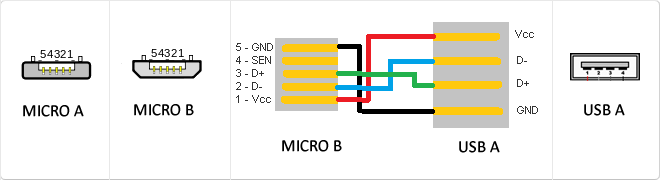
\includegraphics[width=15cm]{./img/micro-usb-type}
\caption{Połączenie przewodów w micro-USB}
\end{figure}

%
% USB ON THE GO ??
%
\section{Historia}
USB zapoczątkowało w 1994 siedem firm: Compaq, DEC, IBM, Intel, Microsoft, NEC, Nortel. Celem było uproszczenie podłączenia zewnętrznych urządzeń do komputera zastępując stare złącza w płytach głównych wprowadzając rozwiązania na problemy znalezione w starych oraz upraszczając software.
Pierwszy układ scalony wspierający USB został wyprodukowany przez Intel 1995r.
\newline

\subsection{USB1.x}
Pierwsza oficjalna wersja standardu USB została wydana w styczniu 1996r. USB1.0 charakteryzowała prędkość 1,5 Mbit/s (Low Speed) oraz 12 Mbit/s (Full Speed). Nie pozwalał jednak na używanie przedłużaczy kabli, wynikało to z limitów zasilania. Powstało kilka wypuszczono na rynek na chwile przed wydaniem standardu USB1.1 w sierpniu 1998r. W USB1.1 poprawiono kilka błędów znalezionych w USB1.0 i był to pierwszy standard, który został oficjalnie zaimplementowany w standardowych komputerach osobistych.
\subsection{USB2.0}
USB2.0 zostało wydane w kwietniu 2000r. udostępniając maksymalny przesył sygnału rzędu 480 Mbit/s (60MB/s) nazwany High Speed (USB1.x za pomocą Full Speed umożliwiał przesył rzędu 12Mbit/s). Biorąc pod uwagę zależności dostępu do magistrali przepustowość High Speed ogranicza się do 280 Mbit/s (35 MB/s).


Przyszłe modyfikacje do specyfikacji USB zostały zaimplementowane przez "Engineering Change Notitices" (ECN). Najważniejsze z ECNów zostały dołączone do specyfikacji USB2.0 dostępnej na stronie internetowej USB.org.
\newline
Przykłady ECNow:
\newline
Złącze Mini-A oraz Mini-B: wydane w październiku 2000r.
\newline


\subsection{USB3.0}

Standard USB3.0 został wydany w listopadzie 2008r. definiujący zupełnie nowy tryb "SuperSpeed". Port USB zwyczajowo jest w kolorze niebieskim i kompatybilny z urządzeniami USB2.0 oraz kablami.
\newline
Dokładnie 17 listopada 2008r. ogłoszono iż specyfikacja dla wersji 3.0 została całkowicie ukończona i została zaakceptowana przez "USB Implementers Forum" (USB-IF), czyli głównej instytucji zajmującej się specyfikacjami standardu USB. To pozwoliło na szybkie udostępnienie standardu deweloperom.
\newline
Nowa magistrala "SuperSpeed" dostarcza czwarty typ transferu z możliwością przesyłania sygnału z prędkością 5GBit/s, ale poprzez użycie kodowania 8b/10b przepustowość wynosi 4Gbit/s. Specyfikacja uznaje za zasadne osiągniecie prędkości w okolicach 3,2 Gbit/s (400 MB/s) co w założeniach powinno się zwiększać wraz z rozwijaniem hardwaru. Komunikacja odbywa się w obu kierunkach dla SuperSpeed (kierunek nie jest naprzemienny i nie jest kontrolowany przez hosta, jak to ma miejsce do wersji USB2.0).
\newline
Podobnie jak w poprzednich wersjach standardu, porty USB3.0 działają dwóch wariantach zasilania: niskiego poboru mocy (low-power: 150mA) oraz wysokiego poboru mocy (high-power: 900mA). Zapewniając odpowiedni jednocześnie pozwalają na przesył danych z prędkością SuperSpeed.
\newline
Została dodatkowo zdefiniowana specyfikacja zasilania (w wersji 1.2 wydana w w grudniu 2010r.) która zwiększała dopuszczalny pobór mocy do 1,5A, ale nie pozwala na współbieżne przesyłanie danych. Specyfikacja wymaga aby fizyczne porty same w sobie były wstanie obsłużyć 5A, ale ogranicza pobór do 1,5 A.

\subsection{USB3.1}
W styczniu 2013r. w prasie pojawiły się informacje o planach udoskonalenia standardu USB3.0 do 10Gbit/s. Zakończyło się to stworzeniem nowej wersji standardu - USB3.1. Wersja ta została wydana 31 lipca 2013r. wprowadzając szybszy typ przesyłania danych zwany "SuperSpeed USB 10 Gbit/s". Zaprezentowano również nowe logo stylizowane na zasadzie "Superspeed+". Standard USB3.1 zwiększył szybkość przesyłu sygnału do 10Gbit/s. Udało się też zredukować obciążenie łącza do 3\% dzięki zmianie kodowania na 128b/132b.
\newline
Przy pierwszych testach prędkośi USB3.1 udało się uzyskać prędkość 7,2Gbit/s.
\newline
Standard USB3.1 jest wstecznie kompatybilny ze standardem USB3.0 oraz USB2.0.


\chapter{Biblioteki}
\label{librariesChapter}
\section{libUSB}
LibUSB jest biblioteką stworzoną w 2007 roku. Napisana w języku C  pozwala na prosty i łatwy dostęp do urządzenia USB. Jest w 100\% przeznaczona dla użytku developera. Biblioteka ma za zadanie ułatwić pisanie aplikacji opartych na komunikacji USB z mikrokontrolerem.
Biblioteka libUSB jest przenośna a co za tym idzie dostępna na wiele platform (Linux, OS X, Windows, Android, OpenBSD, etc.) wraz z niezmiennym API.
Nie są wymagane dodatkowe uprawnienia aby komunikacja z urządzeniem przebiegała poprawnie.
Wspiera standardy USB: 
\begin{itemize}
\item USB1.0 
\item USB1.1 
\item USB2.0 
\item USB3.0
\end{itemize}

Funkcjonalność biblioteki:
\begin{enumerate}

\item wszystkie typy transferu są wspierane (control, bulk, interrupt, isochronous)
\item 2 interfejsy
\begin{enumerate}
\item synchroniczny (prosty)
\item asynchroniczny (bardziej złożony ale bardziej efektywny)
\end{enumerate}
\item stosowanie wątków jest bezpieczne
\item lekka biblioteka z prostym API
\item kompatybilna wstecznie (do wersji libUSB-0.1)
\end{enumerate}

\section{winUSB}

Microsoft Windows począwszy od systemu Windows Vista wprowadził nowy zestaw bibliotek umożliwiający developerom korzystnie z portów USB. WinUSB udostępnia proste API, które pozwala aplikacji na bezpośredni dostęp do portów USB. Został stworzony w gruncie rzeczy dla prostych urządzeń obsługiwanych tylko przez jedną aplikację takich jak urządzenia do odczytu wskaźników pogodowych czy też innych programów które potrzebują szybkiego i bezpośredniego dostępu do portu. WinUSB udostępnia API aby odblokować developera przy pracy z portami USB z poziomu user-mode. W Windowsie 7 USB Media Transfer Protocol (MTP) używa winUSB zamiast poprzednio stosowanych rozwiązań kernela (krenel mode filter driver).

Media Transfer Protocol jest rozszerzeniem PTP (Picture Transfer Protocol) i jest protokołem pozwalającym na przesyłanie atomowe plików audio oraz wideo z oraz do urządzenia. PTP początkowo został zaprojektowany do ściągania zdjęć, obrazów z aparatów cyfrowych, Media Transfer Protocol pozwala na przesyłanie plików muzycznych z cyfrowych urządzeń odtwarzających muzykę oraz pliki video z urządzeń pozwalających na ich odtworzenie.

 
%MTP is a key part of WMDRM10-PD,[1] a digital rights management (DRM) service for the Windows Media platform.

MTP jest częścią frameworku "Windows Media" blisko związanym z odtwarzaczem Windows Media Player. Systemy Windows począwszy od Windows XP SP2 wspierają MTP. Windows XP wymaga Windows Media Player w wersji 10 lub wyższej, późniejsze wersje systemu wspierają już go domyślnie. Microsoft posiada dodatkowo możliwość zainstalowania MTP na wcześniejszych wersjach systemu ręcznie do wersji Microsoft Windows 98.

Twórcy standardu USB ustandaryzowali MTP jako pełnoprawną klasę dla urządzeń USB w maju 2008r.
Od tamtej pory MTP jest oficjalnym rozszerzeniem PTP i współdzieli ten sam kod klasy. %//[odnosnik] odnosnik.



\section{porównanie libUSB oraz winUSB}

\newpage

\chapter{libUSB API}
\label{libUsbChapter}

\section{najważniejsze struktury}
\subsection{libusb\_context}
libusb\_context jest strukturą reprezentującą sesję libusb.
\newline
Koncepcja indywidualnych sesji libusb pozwala aby program mógł korzystać z dwóch bibliotek (lub dynamicznie ładować dwa moduły) z których obie nie zależnie korzystają z libusb. To zapobiega ingerencji (interferencji) pomiędzy dwoma programami używającymi libusb. Dla przykładu libusb\_set\_debug() nie zaingeruje w działanie innego programu korzystającego z libusb, natomiast libusb\_exit() nie wyczyści pamięci używanej przez inny program libusb.
\newline
Sesje tworzone są za pomocą libusb\_init() oraz czyszczone za pomocą libusb\_exit(). Jeśli zagwarantowane jest to, że dana aplikacja jest jedyną która korzysta z libusb, twórca jej nie musi przejmować się kontekstami (strukturą libusb\_context), wystarczy aby przekazywał do wszystkich funkcji, gdzie struktura jest wymagana wartość NULL. Jest to równoważne z użyciem domyślnego kontekstu.

\subsection{libusb\_device\_handle}
Struktura reprezentująca uchwyt do urządzenia USB.
\newline
Jest to nieprzejrzysty typ, użycie jest możliwe tylko za pomocą wskaźnika, zazwyczaj dostarczanego za pomocą funkcji libusb\_open().
\newline
Uchwyt do urządzenia USB jest używany do wykonywania operacji wejścia/wyjścia. Po zakończeniu wszystkich operacji należy wywołać libusb\_close().

\section{najważniejsze funkcje}
\subsection{libusb\_init}
Inicjalizacja biblioteki.
\newline
Funkcja musi zostać wywołana przed wywołaniem jakiejkolwiek innej funkcji z biblioteki libUsb.
\newline
Jeśli w argumencie nie zostanie dostarczony żaden wskaźnik (wyjściowy) kontekstu, zostanie stworzony domyślny kontekst. W przypadku jeśli domyślny kontekst już istnieje zostanie on ponownie użyty (bez ponownej inicjalizacji).
\newline
Funkcja zwraca wartość 0 w wypadku powodzenia, w przeciwnym wypadku zwraca kod błędu.
\subsection{libusb\_open\_device\_with\_vid\_pid}
Wygodna funkcja służąca odszukaniu konkretnego urządzenia na podstawie jego vendorId oraz productId (są to parametry charakteryzujące każde urządzenie).
\newline
Ta funkcja jest używana w przypadkach kiedy z góry jest znane vendorId oraz productId. Najczęściej są to przypadki pisania aplikacji aby przetestować jakąś określoną funkcjonalność. Funkcja pozwala uniknąć wywołanie libusb\_get\_device\_list() i dbania o odpowiednie czyszczenie pamięci po liście.
\newline
Pierwszym parametrem jest kontekst uzyskany za pomocą libusb\_init().
\newline
Kolejnymi parametrami są vendorId oraz productId.
\newline
Funkcja zwraca uchwyt do znalezionego urządzenia, lub NULL w wypadku kiedy nie może znaleźć pożądanego urządzenia (o podanym productId oraz vendorId) lub błędu.
\subsection{libusb\_kernel\_driver\_active}
Funkcja sprawdzająca czy sterownik jądra kernela jest aktywny na interfejsie.
\newline
W wypadku kiedy sterownik jądra jest aktywny nie możliwe jest zgłoszenie użycia interfejsu, a co za tym idzie libUSB nie może wykonać operacji wejścia/wyjścia.
\newline
Funkcjonalność jest nie dostępna w systemie Windows.
\newline
Do funkcji należy przekazać uchwyt do urządzenia oraz numer interfejsu.
\newline
Funkcja zwraca wartość 0, jeśli żaden sterownik jądra nie jest aktywny, wartość 1 w wypadku jeśli istnieje aktywny sterownik jądra.
\newline
W wypadku błędów: LIBUSB\_ERROR\_NO\_DEVICE jeśli urządzenie zostanie odłączone, LIBUSB\_ERROR\_NOT\_SUPPORTED dla platform, gdzie funkcjonalność nie jest wspierana oraz inny kod błędu w wypadku innego błędu.
\subsection{libusb\_detach\_kernel\_driver}
Dzięki funkcji możliwe jest odłączenie sterownika jądra kernela od interfejsu.
\newline
Sukces operacji umożliwi zgłoszenie użycia interfejsu i wykonanie operacji wejścia/wyjścia.
\newline
Funkcjonalność nie jest dostępna dla systemu Windows.
\newline
Parametrami są uchwyt do urządzenia oraz numer interfejsu.
\newline
Funkcja zwraca wartość 0 w momencie powodzenia, LIBUSB\_ERROR\_NOT\_FOUND jeśli żaden sterownik nie był aktywny, LIBUSB\_ERROR\_INVALID\_PARAM jeśli interfejs nie istniej, LIBUSB\_ERROR\_NO\_DEVICE jeśli urządzenie zostało odłączone, LIBUSB\_ERROR\_NOT\_SUPPORTED dla platform, gdzie funkcjonalność nie jest wspierana lub inny kod błędu w wypadku inne błędu.
\subsection{libusb\_claim\_interface}
Dzięki funkcji libusb\_claim\_interface() możliwe jest zgłoszenie użycia danego interfejsu dla danego urządzenia.
\newline
Wywołanie funkcji jest wymagane przed wykonaniem operacji wejścia/wyjścia dla dowolnego punktu końcowego interfejsu.
\newline
Jest dozwolone wywołanie funkcji dla interfejsu już wcześniej zgłoszonego, w tym wypadku zostanie zwrócona wartość 0 bez wykonywania żadnych operacji.
\newline
W wypadku jeśli zmienna auto\_detach\_kernel\_driver jest ustawiona na wartość 1 dla danego urządzenia (zmienna ustawiana za pomocą funkcji: libusb\_set\_auto\_detach\_kernel\_driver()) sterownik jądra zostanie odłączony (jeśli to konieczne), w przypadku niepowodzenia zostanie zwrócony błąd odłączenia.
\newline
Sama procedura wewnątrz funkcji nie jest skomplikowana, nie wymaga wysyłania czegokolwiek po magistrali. Są to proste instrukcje mówiące systemowi operacyjnemu iż aplikacja chce korzystać z danego interfejsu.
\newline
Nie jest to funkcja blokująca.
\newline
Parametrami są uchwyt do urządzenia oraz numer interfejsu zgłaszanego.
\newline
Wartość 0 zostaje zwrócona w wypadku powodzenia operacji.
\newline
W wypadku niepowodzenia kody błędu t.j. LIBUSB\_ERROR\_NOT\_FOUND jeśli podany interfejs nie istnieje, LIBUSB\_ERROR\_BUSY jeśli inny program lub sterownik zarezerwował dany interfejs, LIBUSB\_ERROR\_NO\_DEVICE jeśli urządzenie zostało odłączone oraz inne.
\subsection{libusb\_bulk\_transfer}
Dzięki funkcji możliwy jest przesył większej grupy danych.
\newline
Kierunek jest określony na podstawie bitów kierunkowych punktu końcowego interfejsu.
\newline
Dla odczytu, jeden z parametrów określa ilość danych jaka jest spodziewana przy odczycie. Jeżeli odebrana zostanie mniejsza ilość danych niż oczekiwana, funkcja po prostu zwróci te dane wraz z dodatkowym parametrem określającym ilość otrzymanych danych. Istotne przy odczycie jest to aby sprawdzić czy ilość oczekiwanych danych jest taka jak odczytana.
\newline
W wypadku zapisu również należy sprawdzić czy ilość danych wysłanych pokrywa się z ilością danych skierowaną do wysyłki.
\newline
Wskazana jest również weryfikacja ilości danych wysłanych/odebranych w wypadku wystąpienia timeoutu (funkcja zwróci kod błędu określający timeout). libUSB może podzielić wysyłane dane na mniejsze części i timeout może wystąpić po wysłaniu kilku z nich. Ważne jest to, że nie oznacza to iż nic nie zostało wysłane/odebrane, dlatego należy sprawdzić ilość elementów wysłanych/odebranych i dostosować odpowiednio kolejne kroki.
\newline
Funkcja przyjmuje następujące parametry: uchwyt urządzenia z którym aplikacja będzie się komunikować, adres punktu końcowego interfejsu po którym będzie odbywała się komunikacja, wskaźnik do pamięci danych która ma zostać przetransferowana (w wypadku zapisu) lub odebrana (w wypadku odczytu), ilość danych do wysłania (w przypadku zapisu) lub oczekiwana ilość danych do odebrania (w przypadku odczytu), ilość danych przetransferowanych (w obu przypadkach), maksymalna długość czasu na wykonanie operacji, dla nieograniczonego należy użyć wartości równej 0.
\newline
W przypadku poprawności działania funkcja zwraca wartość 0 oraz ilość przetransferowanych danych przekazanych do funkcji za pomocą wskaźnika.
\newline
W przeciwnym wypadku funkcja zwraca: LIBUSB\_ERROR\_TIMEOUT jeśli transfer przekroczył określony czas, LIBUSB\_ERROR\_PIPE jeśli wystąpił błąd związany z punktem końcowym, LIBUSB\_ERROR\_OVERFLOW jeśli urządzenie wysłało więcej danych niż przewidziane w buforze, LIBUSB\_ERROR\_NO\_DEVICE jeśli urządzenie zostało odłączone oraz inne.
\subsection{libusb\_release\_interface}
Funkcja zwalnia rezerwacje wcześniej zgłoszonego interfejsu za pomocą funkcji libusb\_claim\_interface().
\newline
Zwolnienie wszystkich interfejsów jest wymagane przed zamknięciem urządzenia.
\newline
Nie jest to blokująca funkcja.
\newline
W wypadku jeśli zmienna auto\_detach\_kernel\_driver jest ustawiona na wartość 1 dla danego urządzenia (zmienna ustawiana za pomocą funkcji: libusb\_set\_auto\_detach\_kernel\_driver()) sterownik jądra zostanie ponownie podłączony zaraz po zwolnieniu interfejsu.
\newline
Parametrami są: uchwyt urządzenia oraz numer interfejsu dla niego poprzednio zarezerwowanego.
\newline
Metoda zwraca 0 gdy wszystkie operacje się powiodą.
\newline
W przeciwnym wypadku zwraca: LIBUSB\_ERROR\_NOT\_FOUND jeśli interfejs nie został poprzednio zarezerwowany (zgłoszony do użycia), LIBUSB\_ERROR\_NO\_DEVICE jeśli urządzenie zostało odłączone oraz inne.
\subsection{libusb\_close}
Zwalnia uchwyt do urządzenia.
\newline
Funkcja powinna być wołana na wszystkich używanych uprzednio uchwytach.
\newline
Funkcja pokrótce niszczy referencje stworzoną za pomocą libus\_open() dla danego urządzenia.
\newline
Jest to funkcja nie blokująca.
\newline
Parametrem jest uchwyt przeznaczony do zamknięcia.

\subsection{libusb\_exit}
Funkcja zamyka dostęp do biblioteki.
\newline
Powinna być wołana po zamknięciu wszystkich otwartych urządzeń ale przed zakończeniem działania programu.
\newline
Parametrem jest contekst który ma zostać zamknięty, w wypadku wartości NULL wybierany jest domyślny.

%% asyn interface
\subsection{libusb\_alloc\_transfer}
Funkcja przygotowuje transfer z wyspecyfikowaną ilością 	izochronicznych deskryptorów pakietów.
\newline
Funkcja zwraca uchwyt do zainicjalizowanego transferu. Kiedy wszystkie operacje zostaną na nim wykonane należy wywołać libusb\_free\_transfer().
\newline
Transfer przygotowywany dla nie izochronicznego punktu końcowego należy wywoływać z wartością zero jako ilość izochronicznych pakietów.
\newline
Dla transferów izochronicznych wymagane jest podanie prawidłowej wartości deskryptorów pakietów jakie mają zostać zalokowane w pamięci. Zwracany transfer nie jest domyślnie zainicjalizowany jako izochroniczny, wymagane dodatkowo jest ustawienie pola libusb\_iso\_packets oraz type.
\newline
Alokowanie transferu jako izochroniczny (z podana ilością deskryptorów pakietów do zalokowania) a następnie używanie transferu jako nie izochroniczny jest w 100\% bezpieczne ale pod warunkiem jeśli pole num\_iso\_packets jest ustawione na zero oraz pole type jest ustawione prawidłowo.
\newline
Funkcja jako prametr przyjmuje ilość izochronicznych deskryptorów pakietów.
\newline
Zwracaną jest zalokowany transfer lub NULL w wypadku błędu.
\subsection{libusb\_fill\_bulk\_transfer}
Funkcja pozwala na łatwe przygotowanie struktury libusb\_transfer na transfer masowy.
\newline
Parametrami są:
\begin{itemize}
\item uchwyt do ustawianego transferu
\item uchwyt do urządzenia dla którego ustawiany jest transfer
\item adres punktu końcowego gdzie dane mają zostać wysłane
\item bufor danych do wysłania/odebrania
\item długość (wielkość) wysyłanych/odbieranych danych
\item wskaźnik do funkcji która ma się wywołać po zakończeniu transferu (callback)
\item dodatkowe dane, które programista może opcjonalnie wysłać do funkcji wywołanej po zakończeniu transferu 
\item czas oczekiwania w milisekundach na zakończenie transferu
\end{itemize}
\subsection{libusb\_submit\_transfer}
Funkcja wykonuje podany (ustawiony) transfer.
\newline
Funkcja wykonuje operacje na interfejsie po czym bezzwłocznie kończy działanie.
\newline
Jedynym parametrem jaki przyjmuje funkcja jest wskaźnik do transferu jaki ma zostać wykonany.
\newline
W wypadku kiedy wszystko się powiedzie funkcja zwraca wartość równą 0, w pozostałych przypadkach zwraca kod błędu tj. LIBUSB\_ERROR\_NO\_DEVICE w wypadku kiedy urządzenie nie jest podłączone, LIBUSB\_ERROR\_BUSY w przypadku jeśli akcja została już wykonana, LIBUSB\_ERROR\_NOT\_SUPPORTED jeśli flagi transferu (ustawienia) są nie wspierane przez system operacyjny oraz inne.
\subsection{libusb\_free\_transfer}
Funkcja odpowiada za zwolnienie pamięci zajętą przez strukturę libusb\_transfer
\newline
Funkcja ta powinna być zawołana dla wszystkich transferów zaalokowanych przez libus\_alloc\_transfer().
\newline
Jeśli dodatkowo flaga LIBUSB\_TRANSFER\_FREE\_BUFFER jest ustawiona oraz bufor transferu jest nie zerowy, pamięć po nim zostanie również zwolniona za pomocą standardowej funkcji alokującej (np. free()).
\newline
Dozwolone jest zawołanie funkcji z parametrem równym NULL, w takim przypadku funkcja zakończy się bez błędu (ale nic nie zostanie zwolnione).
\newline
Nie dozwolone jest zwalnianie pamięci po nie zakończonym (aktywnym) jeszcze transferze, czyli takim który wystartował ale jeszcze nie wywołany został callback do niego (lub timeout).
\newline
Parametrem funkcji jest wskaźnik do transferu do zwolnienia.

%---------
\chapter{Mikrokontroler}
\label{microcontrollerChapter}
\begin{figure}[h]
\centering
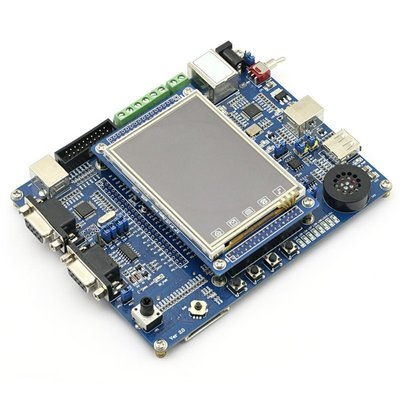
\includegraphics{./img/landTiger}
\caption{Mikrokontroler LandTiger wraz z wyświetlaczem}
\end{figure}

Mikrokontroler LandTiger oparty na LPC1768 został wyprodukowany przez firmę PowerMCU i można ją zakupić od wielu dostawców na eBay lub innych serwisach świadczących usługi zakupów przez internet. Średni koszt waha się w granicach \$70 za płytkę wraz z wyświetlaczem LCD 3,2 cala o rozdzielczości 320x240 pikseli, z zasilaczem oraz zestawem kabli.
\newline
Funkcjonalności:
\begin{enumerate} [label=(\alph*)]
\item 2 porty RS232, jeden z nich wspiera ISP (In-system Programming)
\item 2 interfejsy magistrali CAN (Controller Area Network)
\item interfejs RS485
\item interfejs Ethernetowy RJ45-10/100M 
\item przetwornik cyfrowo-analogowy (DAC) wraz wmontowanym głośnikiem (wyjściem interfejsu) oraz sterownikiem dźwięku (LM386)
\item przetwornik analogowo-cyfrowy (ADC) wraz z wbudowanym potencjomentrem (wejściem interfejsu).
\item Kolorowy 3,2 cala (lub 2,8 cala) dotykowy wyświetlacz LCD o rozdzielczości 320x240 pikseli. 
\item interfejs USB2.0 (USB Host oraz USB Device)
\item interfejs kard SD/MMC
\item interfejs I2C połączony z 2Kbit pamięcią EEPROM
\item interfejs SPI połączony z 16Mbit pamięcią flash
\item 2 user keys, 2 function keys
\item 8 diód typu LED
\item pięciokierunkowy joystick
\item wsparcie dla pobierania ISP
\item pobieranie z użyciem JTAG, interfejs dla debugowania
\item zintegrowany emulator kompilacji JLINK - wspiera możliwość debugownia online (po kablu USB podłączonym do PC) dla środowisk deweloperskich tj. KEIL, IAR, CooCox i innych
\item dodatkowe 5V port zasilający (możliwe jest też za pomocą portu USB 
\end{enumerate}

\begin{figure}[h]
\centering
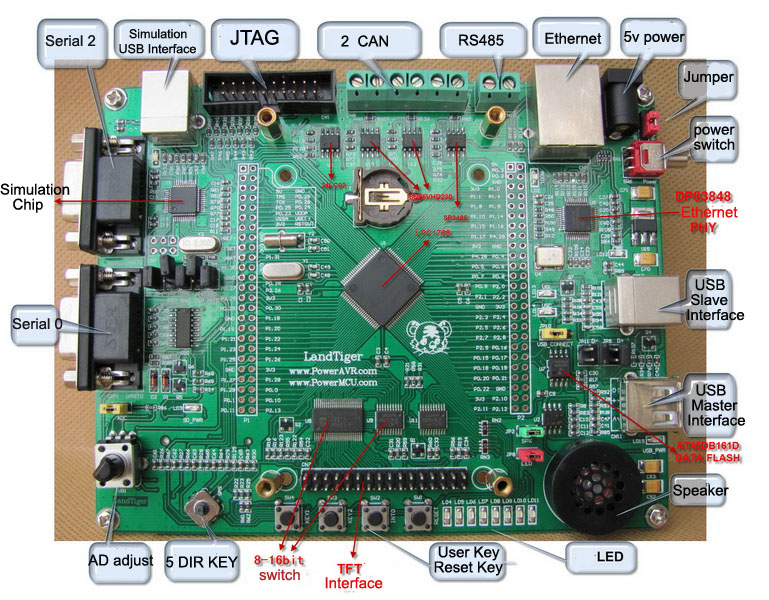
\includegraphics{./img/landTiger3}
\caption{Mikrokontroler LandTiger wraz z opisem poszczególnych elemetnów}
%example\caption{Krzywa plastyczności wyrażająca zależność odkształcenia od naprężenia podczas rozciągania materiału ciągliwego \cite{bib7}} 
\end{figure}
LandTiger jest oparty na LPC1768. Wbudowany hardware wspiera ISP aby umożliwić załadowanie kodu (z użyciem bin2hex oraz flashmagic).
\newline
Alternatywą jest to, że kod może zostać załadowany za pomocą emulatora JLINK JTAG/SWD lub za pomocą zewnętrznego urządzenia JTAG.
\newline
Port COM1 (UART0) wspiera komunikacje z PC w obie strony. Wszelkie funkcje portu USB są wspierane z minimalnymi zmianami w oprogramowaniu. Podobnie jest z Ethernetem, z niewielkimi  zmianami w oficjalnym kodzie dla LPC1768 kod jest w stanie się uruchomić na LandTigerze.
\newline
Wyświetlacz LCD jest oparty na kontrolerze SSD1289. Wyświetlacz może zostać odłączony od płyty. Używa 8-bitowej magistrali \(P2_0..P2_7\). Kontroler ekranu dotykowego jest dostarczony razem z modułem wyświetlacza. Interfejs pomiędzy ekranem dotykowym a LPC1768 jest możliwy dzięki SPI.
\newline
Główne różnice pomiędzy LandTigerem a LPC1768:
\begin{enumerate} [label=(\alph*)]
\item płyta po podłączeniu do PC nie pokazuje się jako zewnętrzne urządzenie magazynujące
\item aby ściągnąć nowe pliki binarne należy użyć ISP lub JTAG
\item brak wsparcia dla serialowego portu po linku USB, należy używać RS232 lub portu USB
\item brak wsparcia dla logicznego systemu plików
\item brak wsparcia dla 4 diód typu LED (istnieje możliwość użycia inncyh).
\end{enumerate}

\chapter{Synchroniczne przesyłanie danych}
Jedną z metod dostępnych, która została użyta w przygotowaniu tej pracy jest wykorzystanie synchronicznych możliwości przesyłu danych z wykorzystaniem libUSB.

\section{zalety}
\begin{itemize}
\item duża kontrola nad wysyłanymi/odbieranymi danymi
\item debugowanie jest mało skomplikowane w porównaniu do asynchronicznego przesyłania danych
\end{itemize}
\section{wady}
\begin{itemize}
\item możliwości prędkości są mocno ograniczone poprzez funkcje blokujące

\end{itemize}
\section{implementacja}
Implementacja opiera się na wykorzystaniu prostych podstawowych funkcji z biblioteki libUsb.

\subsection{Funkcja getContext}
W listingu \ref{lst:getContext} przedstawione zostało ciało funkcji getContext().
\newline
Funkcja nie przyjmuje żadnego argumentu, natomiast zwraca kontekst który jest później przekazywany do wielu metod jako argument. W rozdziale \ref{libUsbChapter} wspomniane zostało iż możliwe jest używanie kontekstu domyślnego, wtedy zamiast tej funkcji i wartości zwracanej (pozyskanego kontekstu) w każdym użyciu uzyskanego przez getContext() wskaźnika należałoby wpisać wartość NULL. 
\newline
Aby używać domyślnego kontekstu należy mieć pewność iż aplikacja/wątek jest jedynym użytkownikiem libUSB.
\newline
\begin{lstlisting}[caption={Funkcja getContext()},label={lst:getContext}]
libusb_context* getContext()
{
	libusb_context* ctx = NULL;
	int r = libusb_init(&ctx);
	if(r < 0) {
		std::cout<<"Init Context error Error "<< r <<std::endl;
		return NULL;
	}
	return ctx;
}
\end{lstlisting}
\subsection{Funkcja getDeviceHandler}
Funkcja nie przyjmuje żadnego argumentu. Zwracany jest uchwyt do LandTiger'a, lub wartość NULL w wypadku błędu (np. braku podłączonego i uruchomionego mikrokontrolera).
Ciało funkcji zostało przedstawione w Listingu \ref{lst:getDeviceHandle}
\begin{lstlisting}[caption={Funkcja getDeviceHandler()},label={lst:getDeviceHandle}]
libusb_device_handle* getDeviceHandle(libusb_context* ctx)
{
	libusb_device_handle* dev_handle = libusb_open_device_with_vid_pid(ctx, LAND_TIGER_VID, LAND_TIGER_PID);
	if(dev_handle == NULL)
		std::cout<<"Cannot open device"<<std::endl;
	else
		std::cout<<"Device Opened"<<std::endl;

	return dev_handle;
}
\end{lstlisting}
\subsection{Funkcja proceedWithInitLibUsb}
Funkcja odpowiedzialna za dokończenie procedur inicjalizacyjnych. Ciało funkcji zostało przedstawione w Listingu \ref{lst:proceedWithInitLibUsb}. Funkcja sprawdza dodatkowo czy sterownik jądra kernela jest aktywny, dla platformy Windows funkcja zwróci wartość LIBUSB\_ERROR\_NOT\_SUPPORTED (!= 1) i zachowa się analogicznie jak w wypadku nie aktywnego sterownika w systemie UNIX (warunek bedzie nie spełniony).
\newline
Kolejnym krokiem jest rezerwacja przez program konkretnego interfejsu za pomocą funkcji libusb\_claim\_interface.
\begin{lstlisting}[caption={Funkcja proceedWithInitLibUsb()},label={lst:proceedWithInitLibUsb}]
int proceedWithInitLibUsb(libusb_device_handle* dev_handle, libusb_context* ctx)
{
		
	if(libusb_kernel_driver_active(dev_handle, 0) == 1) { //find out if kernel driver is attached
		std::cout<<"Kernel Driver Active"<<std::endl;
		if(libusb_detach_kernel_driver(dev_handle, 0) == 0) //detach it
			std::cout<<"Kernel Driver Detached!"<<std::endl;
	}
	int status = libusb_claim_interface(dev_handle, 1);
	if(status < 0) 
	{
		std::cout<<"Cannot Claim Interface"<<std::endl;
		return 1;
	}
	std::cout<<"Claimed Interface"<<std::endl;

	return 0;
}
\end{lstlisting}
\subsection{Funkcja doTest}
Funkcja w całości przedstawiona w Listingu \ref{lst:doTest} i jest odpowiedzialna za wykonanie podstawowego pomiaru czasu przepływu danych w obie strony pomiędzy PC a mikrokontrolerem.
\newline
Została zaprojektowana w taki sposób aby konkretny bufor danych został wysłany oraz odebrany określoną ilość razy i zwrócony przedział czasowy w jakim udało się to uzyskać. Powodem wysyłania/odbierania danych określoną ilość razy jest fakt dość sporych ograniczeń jeśli chodzi o chip wbudowany w płytę LandTiger.
\begin{lstlisting}[caption={Funkcja doTest()},label={lst:doTest}]
int doTest(libusb_device_handle* dev_handle, int bufforSize, int count, double* timeResult)
{
	unsigned char *data_out = new unsigned char[bufforSize]; //data to write
	unsigned char* data_in = new unsigned char[bufforSize];
	generateSymulatedData(data_out, bufforSize);
	int howManyBytesIsSend; 
	int howManyBytesReceived;

	time_t start_t, end_t;
    *timeResult = 0;

	
	time(&start_t);
	for(int i = 0; i < count; ++i)
	{
		int sendStatus = libusb_bulk_transfer(dev_handle, (2 | LIBUSB_ENDPOINT_OUT), data_out, bufforSize, &howManyBytesIsSend, 0); 
		if(sendStatus == 0 && howManyBytesIsSend == bufforSize)
		{
			//here was printing data for debugging only
		}
		else
		{
			std::cout<< "Write Error" << std::endl;
			delete [] data_out;			
			return 1;
		}
		
		
		int readStatus = libusb_bulk_transfer(dev_handle, (2 | LIBUSB_ENDPOINT_IN), data_in, bufforSize * sizeof(unsigned char), &howManyBytesReceived, 0);
		if (readStatus == 0 && howManyBytesReceived == howManyBytesIsSend) 
		{
			//here was printing data for debugging only
		} 
		else 
		{
			std::cout << "Read Error: " << readStatus << std::endl;
			delete[] data_in;
			return 1;
		}
		
	}
	time(&end_t);
	*timeResult = difftime(end_t, start_t);
	delete[] data_in;
	delete [] data_out;
	return 0;
}
\end{lstlisting}
\subsection{Funkcja closeLibUsb}
Funkcja przedstawiona w Listingu \ref{lst:closeLibUsb} odpowiada za zwolnienie interfesju oraz zasobów uprzednio zajętych na czas testu.
\begin{lstlisting}[caption={Funkcja closeLibUsb()},label={lst:closeLibUsb}]
int closeLibUsb(libusb_device_handle* dev_handle, libusb_context* ctx)
{
	int status = libusb_release_interface(dev_handle, 1); 
	if(status != 0) {
		std::cout<<"Cannot Release Interface"<<std::endl;
		return 1;
	}
	std::cout<<"Released Interface"<<std::endl;

	libusb_close(dev_handle);
	libusb_exit(ctx); 
	return 0;
}
\end{lstlisting}
\subsection{główny program synchronicznie przesyłający dane}
Kod przedstawiony w Listingu \ref{lst:synchronicMain} doskonale ukazuje prostotę korzystania z libUSB. Użytkownik zobligowany jest do wprowadzenia wielkości bufora danych oraz ilości powtórzeń określających ile razy dany bufor zostanie wysłany do mikrokontrolera. Następnie zostaje wykonana inicjalizacja z użyciem wyżej wymienionych funkcji oraz test główny również opisany powyżej. Całość zostaje zakończona czyszczeniem zarezerwowanych zasobów. W kodzie widoczne są wszelkiego rodzaju komunikaty o błędach oraz przy inicjalizacji aby użytkownik miał świadomość jak wielkich rozmiarów test będzie wykonywany.
\begin{lstlisting}[caption={Funkcja main()},label={lst:synchronicMain}]
int main(int argc, char* argv[])
{
	if(argc < 3) 
	{
		std::cout << "use: libusbtest <bufforSize> <count>" << std::endl;
		std::cout << "Note that max buffer of LandTiger is " << BUFFOR_MAX << "Bytes" << std::endl;
		return 0; 
	}
	
	int bufforSize = atoi(argv[1]);
	if(bufforSize > BUFFOR_MAX) 
	{
		std::cout << "bufforSize is grather than 64B, setting 64 as default" << std::endl;
		bufforSize = BUFFOR_MAX;
	}

	int count = atoi(argv[2]);

	std::cout << "Total size to send/receive: " << bufforSize << " x " << count << " = " << bufforSize * count << " Bytes" << std::endl;
	
	libusb_context *ctx = getContext(); 
	libusb_device_handle* dev_handle = getDeviceHandle(ctx);
	if(ctx == NULL || dev_handle == NULL)
	{
		return 1;
	}
	int initStatus = proceedWithInitLibUsb(dev_handle, ctx);
	if(initStatus != 0) 
	{
		std::cout << "proceedWithInitLibUsb exited with errors!" << std::endl;
		return 1;
	}
	double testResult = 0.;
	int testStatus = doTest(dev_handle, bufforSize, count, &testResult);
	if(testStatus != 0) 
	{
		std::cout << "There was an error during tests!!" << std::endl;
	}
	else
	{
		std::cout << "Sending of: " << bufforSize * count << "Bytes using bufferSize=" << bufforSize << " takes " << testResult << "s." << std::endl;

	}


	if(closeLibUsb(dev_handle, ctx) != 0)
	{
		return 1;
	}

	return 0;
}
\end{lstlisting}

\end{document}